\newcommand{\TabTgtImprovDiskParams}{
\begin{table}[tb]
\centering
\sisetup{
table-number-alignment=center
}
\begin{tabular}{|r|S[table-format=5.1]S[table-format=1.5]S[table-format=3.3]|}
\multicolumn{1}{|L{1.1cm}}{Disk Index} & \multicolumn{1}{|L{1.8cm}}{Beamline Position (mm)} & \multicolumn{1}{L{1.5cm}}{Relative Gyroradius} & \multicolumn{1}{L{2cm}|}{Disk Radius in Simulation} \\
\hline
0 & 19542.0 & 1.09832 & 144.758 \\
1& 19592.1 & 1.11405 & 148.932 \\
2& 19642.2 & 1.13064 & 153.400 \\
3& 19692.3 & 1.14836 & 158.248 \\
4& 19742.4 & 1.16753 & 163.576 \\
5& 19792.5 & 1.18847 & 169.495 \\
6& 19842.6 & 1.21130 & 176.068 \\
7& 19892.7 & 1.23601 & 183.326 \\
8& 19942.8 & 1.26227 & 191.198 \\
9& 19992.9 & 1.28943 & 199.516 \\
10 & 20043.0 & 1.31668 & 208.037 \\
11 & 20093.1 & 1.34304 & 216.451 \\
12 & 20143.2 & 1.36771 & 224.474 \\
13 & 20193.3 & 1.39005 & 231.867 \\
14 & 20243.4 & 1.40984 & 238.518 \\
15 & 20293.5 & 1.42688 & 244.317 \\
16 & 20343.6 & 1.44127 & 249.272 \\
17 & 20393.7 & 1.45330 & 253.450 \\
\hline
\end{tabular}~%
\begin{tabular}{|r|S[table-format=5.1]S[table-format=1.5]S[table-format=3.3]|}
\multicolumn{1}{|L{1.1cm}}{Disk Index} & \multicolumn{1}{|L{1.8cm}}{Beamline Position (mm)} & \multicolumn{1}{L{1.5cm}}{Relative Gyroradius} & \multicolumn{1}{L{2cm}|}{Disk Radius in Simulation} \\
\hline
18 & 20443.8 & 1.46330 & 256.950 \\
19 & 20493.9 & 1.47151 & 259.842 \\
20 & 20544.0 & 1.47823 & 262.219 \\
21 & 20594.1 & 1.48347 & 264.080 \\
22 & 20644.2 & 1.48745 & 265.500 \\
23 & 20694.3 & 1.49056 & 266.612 \\
24 & 20744.4 & 1.49296 & 267.471 \\
25 & 20794.5 & 1.49478 & 268.125 \\
26 & 20844.6 & 1.49612 & 268.604 \\
27 & 20894.7 & 1.49703 & 268.933 \\
28 & 20944.8 & 1.49730 & 269.030 \\
29 & 20994.9 & 1.49730 & 269.030 \\
30 & 21045.0 & 1.49714 & 268.972 \\
31 & 21095.1 & 1.49692 & 268.891 \\
32 & 21145.2 & 1.49671 & 268.817 \\
33 & 21195.3 & 1.49667 & 268.804 \\
34 & 21245.4 & 1.49673 & 268.823 \\
   &         &         &         \\
\hline
\end{tabular}
\caption
[Parameters of the target disks used in the proof of principle simulation.]{
Parameters of the target disks used in the proof of principle simulation.
Since the beamline axis is parallel to the $-z$ direction in the stopping target region, the Z-coordinate can be obtained from the beamline position via: $z=2164-(s-19542)$.
\tablabel{app:tgtImprov:diskParams}}
\end{table}
}

\newcommand{\FigTgtImprovFieldVsBeamline}{
\begin{figure}[tb]
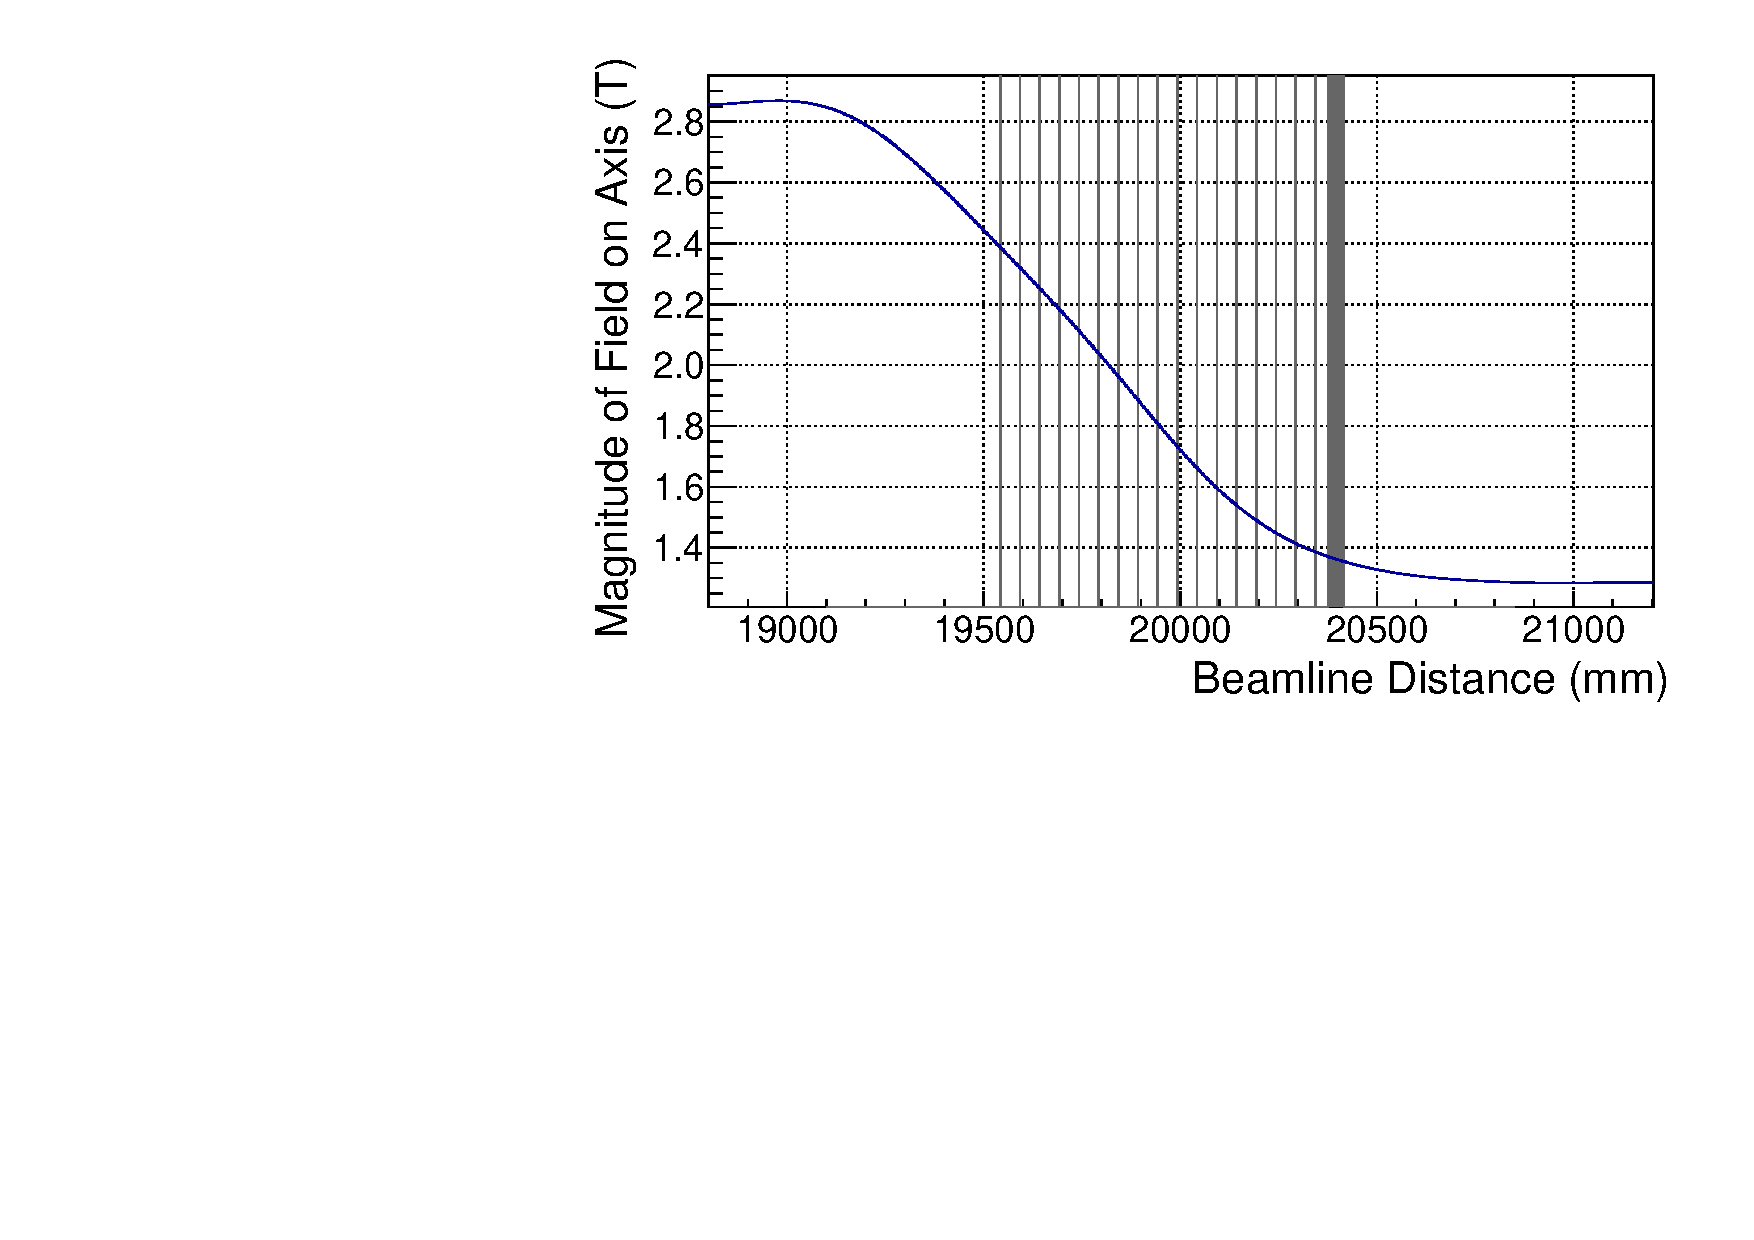
\includegraphics[width=0.9\textwidth,trim=1.0cm 0cm 0.8cm 0,clip]{figs/appendixStopTgtImprov/Plot_FieldMagnitude.pdf}
\caption
[The magnitude of the magnetic field around the stopping target.]{
The magnitude of the magnetic field around the stopping target.
The vertical grey lines indicate the position of the stopping target disks and beam blocker in the target design used in chapter~\sect{sense}.
The muon beam arrives from the left, and signal electrons should leave to the right.
\figlabel{app:tgtImprov:field}}
\end{figure}
}

\newcommand{\FigTgtImprovMirrorVsBeamline}{
\begin{figure}[tb]
\subfloat[][\figlabel{app:tgtImprov:mirror:thetaMin}Minimum Pitch Angle]{%
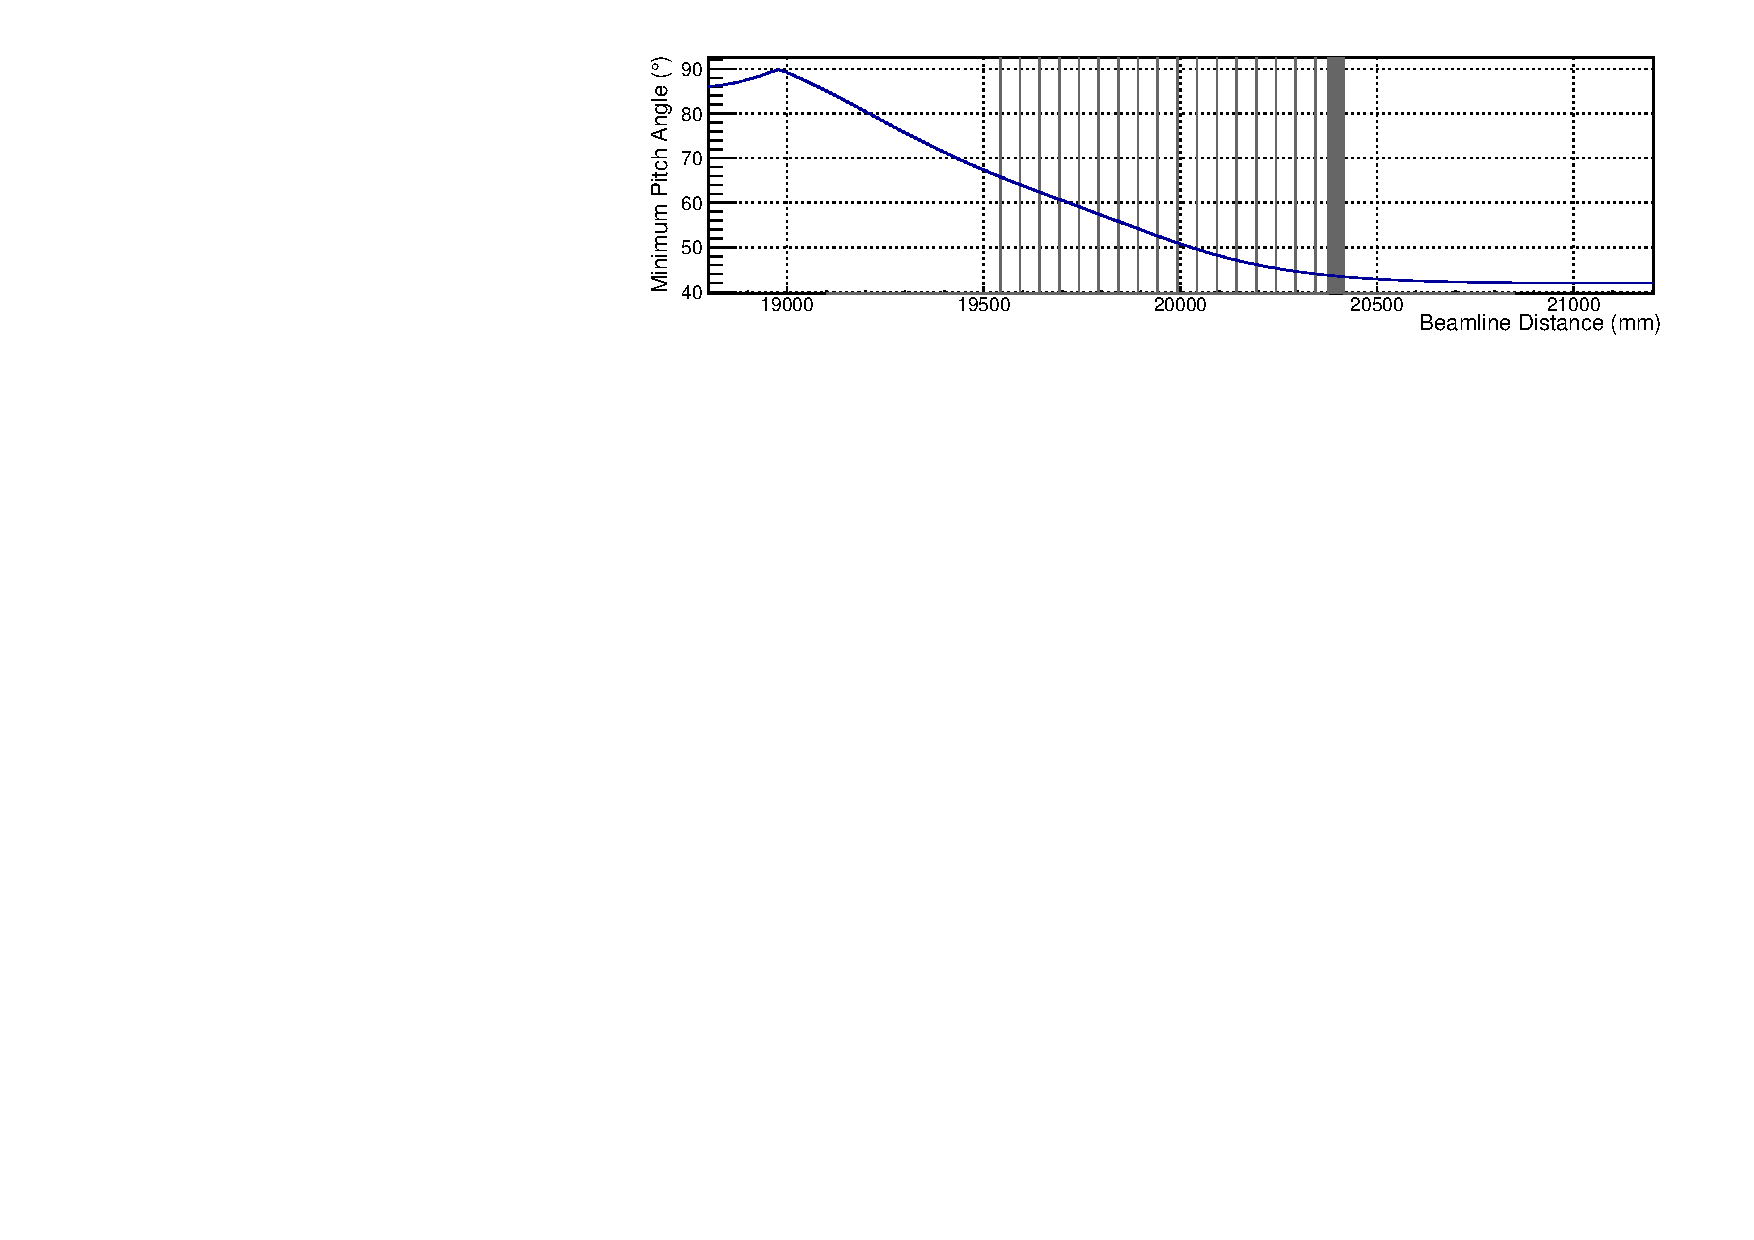
\includegraphics[width=0.9\textwidth,trim=1.5cm 0 0.8cm 0,clip]{figs/appendixStopTgtImprov/Plot_ThetaMin.pdf}}\\
\subfloat[][\figlabel{app:tgtImprov:mirror:phaseSpace}Fraction of Space Which Can be Mirrored]{%
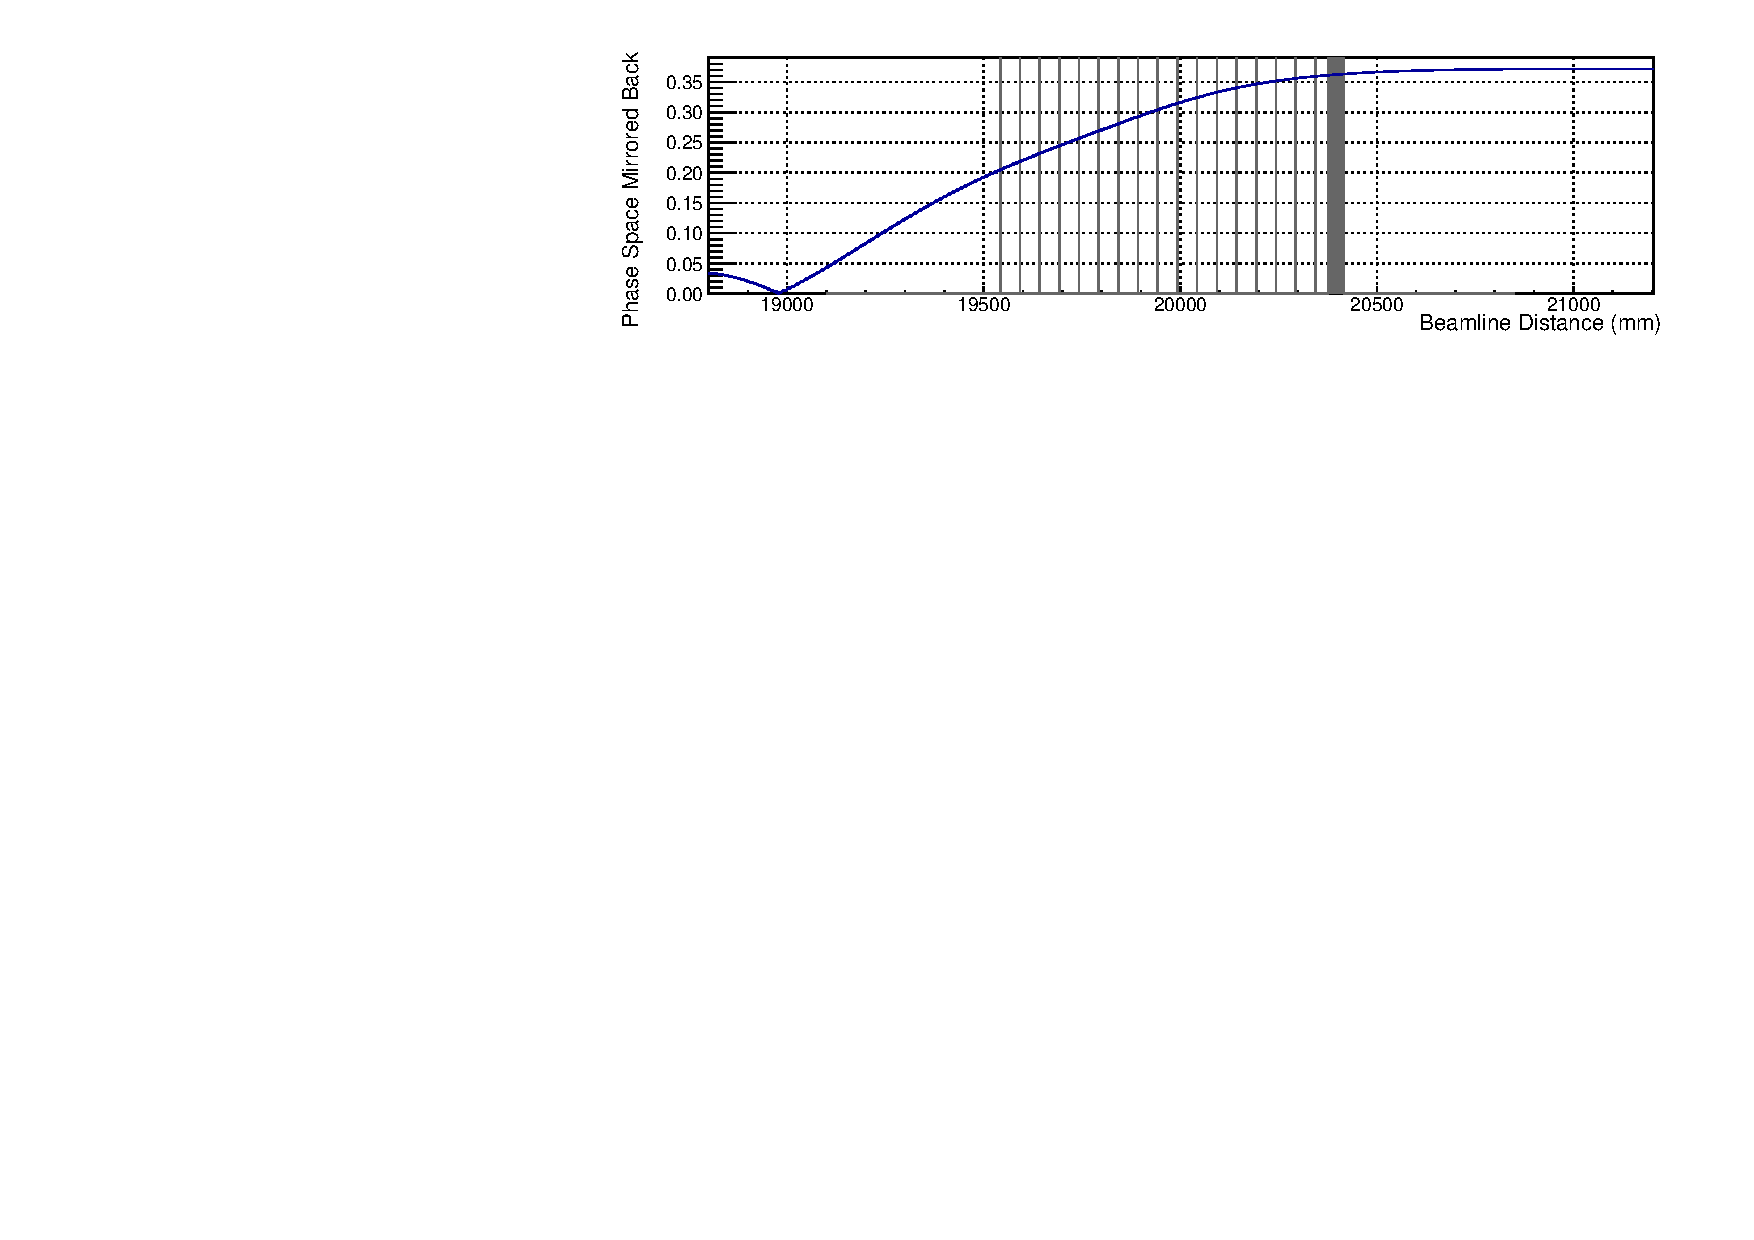
\includegraphics[width=0.9\textwidth,trim=1.5cm 0 0.8cm 0,clip]{figs/appendixStopTgtImprov/Plot_PhaseSpaceFraction.pdf}}
\caption
[The ability for a particle to be mirrored downstream, if it is initially heading upstream at this point.]{
The ability for a particle to be mirrored downstream, if it is initially heading upstream at this point.
For an electron produced at a given point along the beamline, if its pitch angle is too small it will not be mirrored.
The minimum pitch angle is shown in \protect\subref{fig:app:tgtImprov:mirror:thetaMin}.
Since electrons are produced isotropically, this minimum pitch angle can be used to define the fraction of phase space that will be mirrored back, \protect\subref{fig:app:tgtImprov:mirror:phaseSpace}.
\figlabel{app:tgtImprov:mirror}}
\end{figure}
}

\newcommand{\FigTgtImprovGyroradiusVsBeamline}{
\begin{figure}[tb]
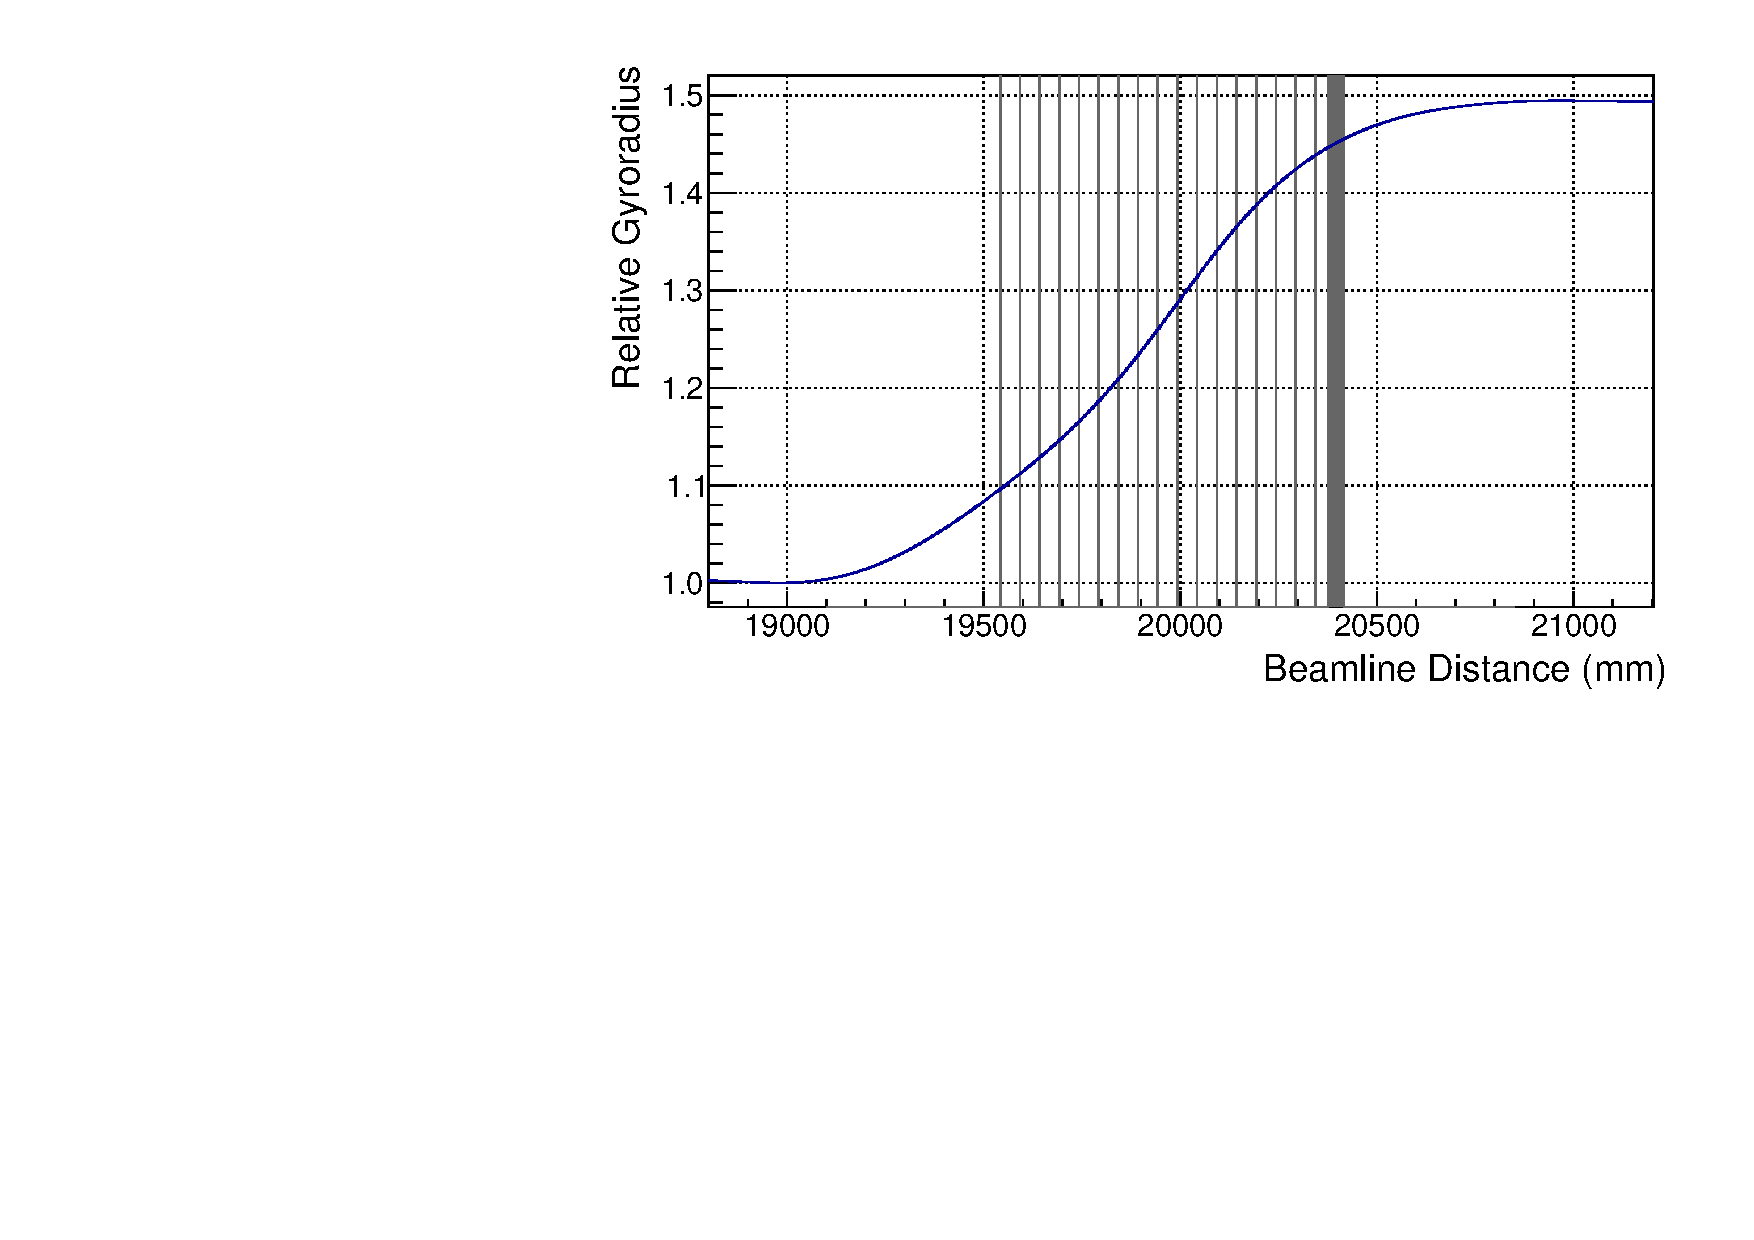
\includegraphics[width=0.9\textwidth,trim=1.2cm 0.2cm 0.8cm 0.2cm,clip]{figs/appendixStopTgtImprov/Plot_GyroradiusGrowth.pdf}
\caption
[Growth in the beam envelope as a function of the distance along the beamline.]{
As the muon beam progresses along the beamline, the beam envelope varies proportional to the square root of the field strength.
The maximum field occurs at the exit of the Torus2 solenoid, with a field strength of about 2.88~T, and this plot shows the relative change in the beam envelope compared to that point.
\figlabel{app:tgtImprov:gyroradius}}
\end{figure}
}

\newcommand{\FigTgtImprovSenseVsBeamline}{
\begin{figure}[tb]
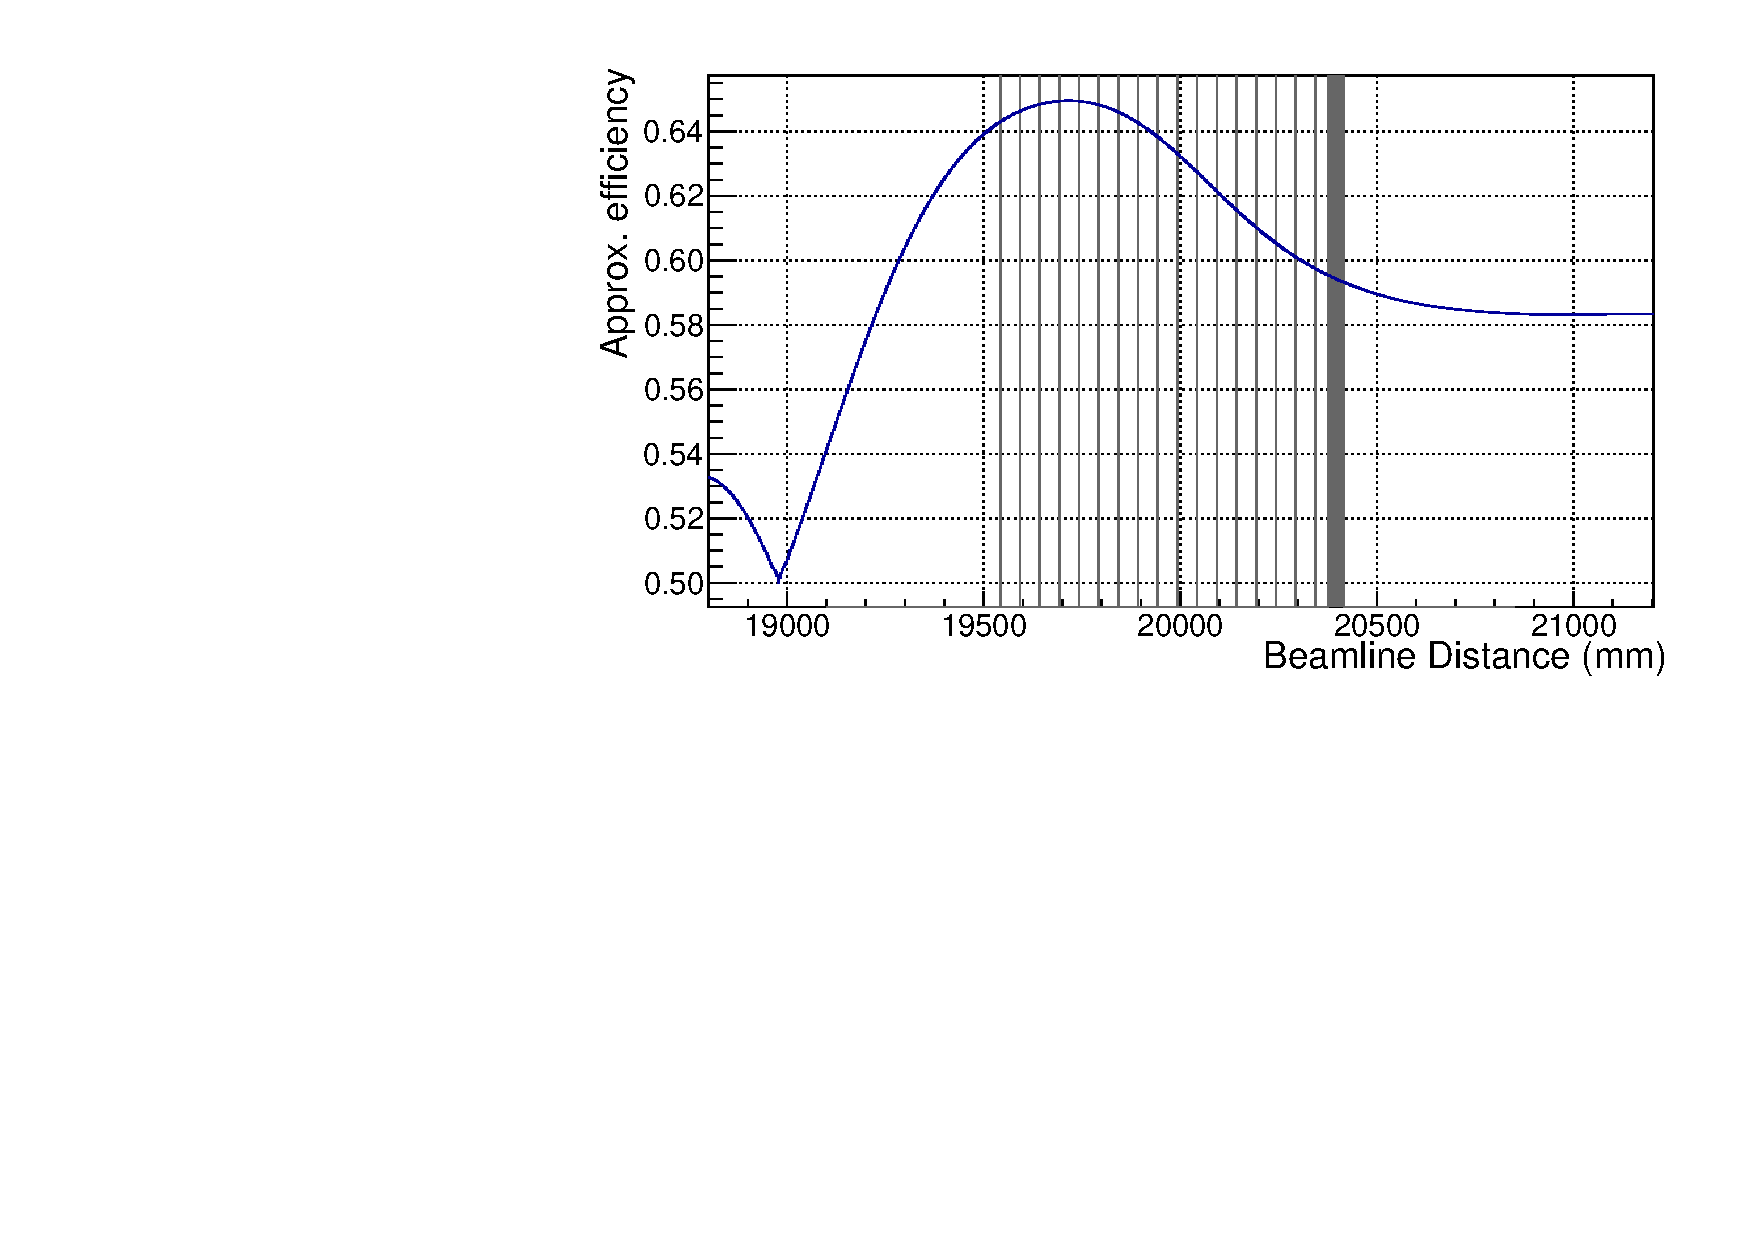
\includegraphics[width=0.9\textwidth,trim=1.1cm 0.3cm 0.8cm 0.3cm,clip]{figs/appendixStopTgtImprov/Plot_ApproxEfficiency.pdf}
\caption
[The effective signal sensitivity achieved by placing a disk of fixed radius at a given location along the beamline.]{
The effective signal sensitivity achieved by placing a disk of fixed radius at a given location along the beamline.
It suggests an optimal target position slightly upstream of the location found in the optimisation chapter, but the difference is easily explained by simplifications in this model.
\figlabel{app:tgtImprov:senseVsBeamline}}
\end{figure}
}

\newcommand{\FigTgtImprovNewGeom}{
\begin{figure}[tb]
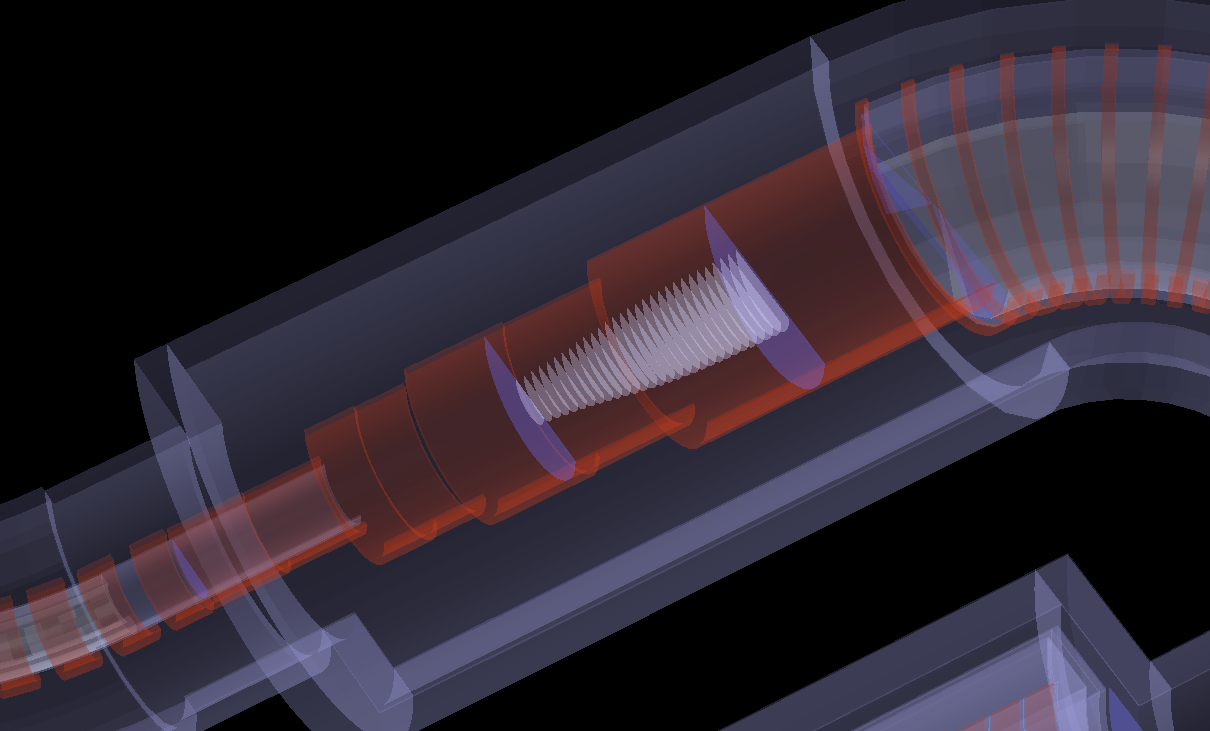
\includegraphics[width=0.7\textwidth]{figs/appendixStopTgtImprov/NewGeometry.png}
\caption
[The new geometry of the stopping target, with the beam blocker removed.]{
The new geometry of the stopping target, with the beam blocker removed.
The blue vertical planes are the virtual monitors used in the simulation and not a physical piece of material.
\figlabel{app:tgtImprov:newGeom}}
\end{figure}
}

\newcommand{\FigTgtImprovMuStops}{
\begin{figure}[ptb]
\begin{minipage}[b]{0.35\textwidth}
\subfloat[][\figlabel{app:tgtImprov:muStops:XZ}Above Target (X-Z)]{%
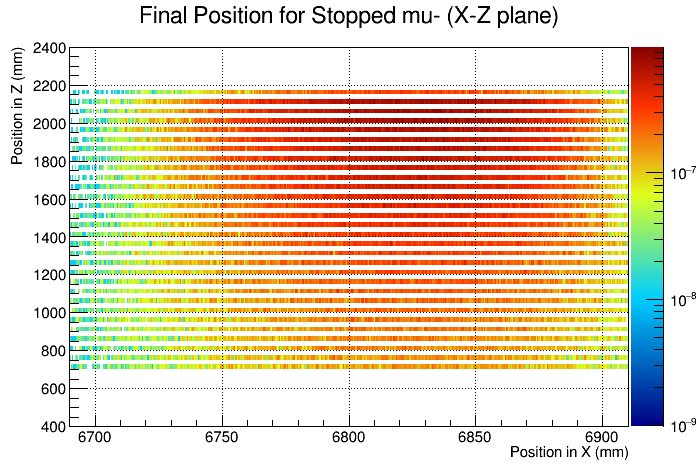
\includegraphics[width=\textwidth,trim=0 0 0 0,clip]{figs/appendixStopTgtImprov/Tidied_Mu_StopPosition_XZ.png}}\\
\subfloat[][\figlabel{app:tgtImprov:muStops:YZ}Side View (Z-Y)]{%
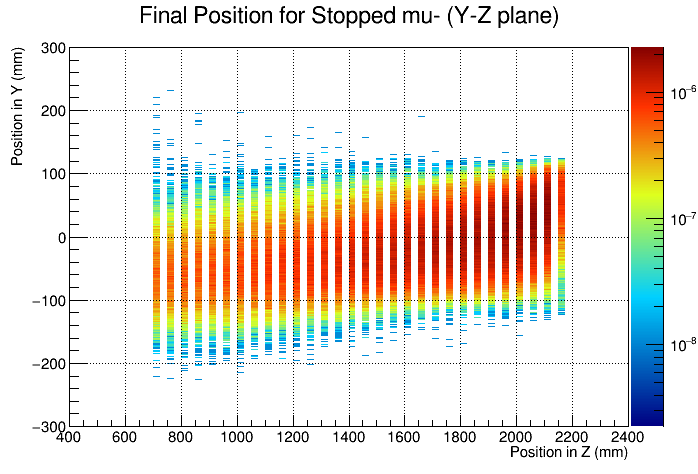
\includegraphics[width=\textwidth,trim=0 0 0 0,clip]{figs/appendixStopTgtImprov/Tidied_Mu_StopPosition_ZY.png}}
\end{minipage}
\subfloat[][\figlabel{app:tgtImprov:muStops:Z}Z Projection]{%
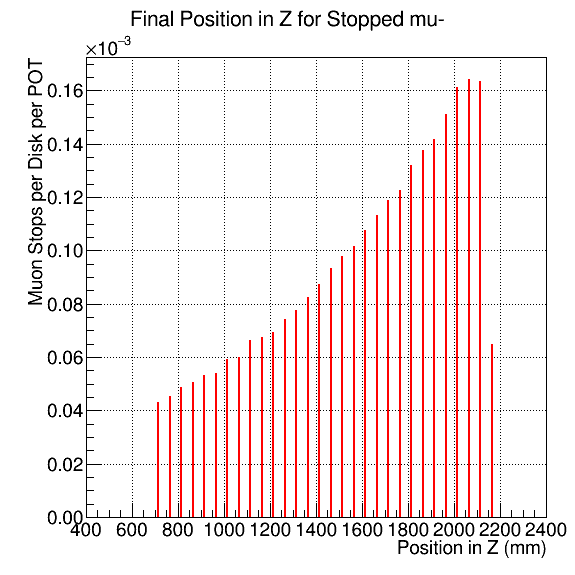
\includegraphics[width=0.5\textwidth,trim=0 0 0 0,clip]{figs/appendixStopTgtImprov/Tidied_Mu_StopPosition_Z.png}}
\caption
[Projections of the muon stopping distribution with the improved target design, to be compared to \fig{sense:stops}.]{
Projections of the muon stopping distribution with the improved target design, to be compared to \fig{sense:stops}.
Although the disks are symmetric, it is clear from \protect\subref{fig:app:tgtImprov:muStops:YZ} how there are fewer muon stops in the upper parts of the disks.
Removing the material there will improve the signal acceptance further.
\figlabel{app:tgtImprov:muStops}}
\end{figure}
}

\newcommand{\FigTgtImprovMuMomentum}{
\begin{figure}[ptb]
\subfloat[][\figlabel{app:tgtImprov:muMomentum:lin}Linear Scale]{%
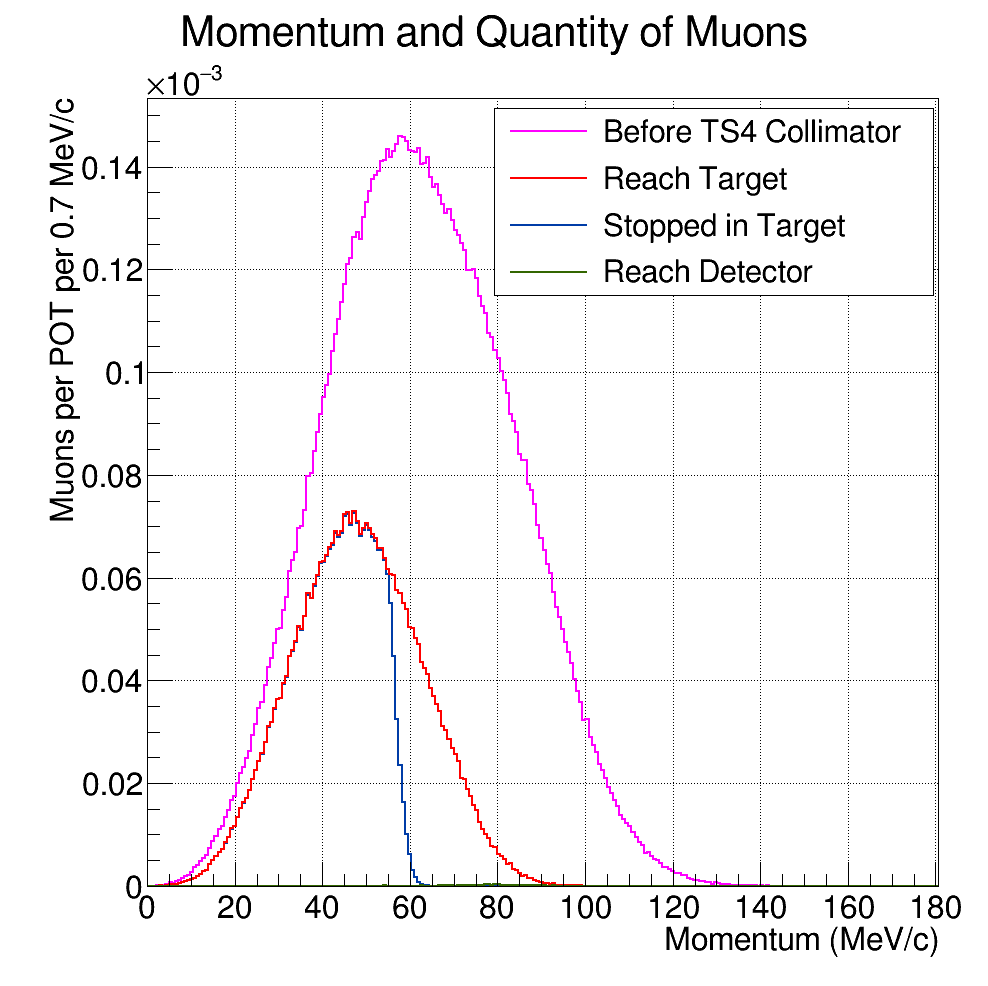
\includegraphics[width=0.49\textwidth,trim=0 0 0 0,clip]{figs/appendixStopTgtImprov/Tidied_muon_momentum_withDetectedMuons_lin.png}}
\subfloat[][\figlabel{app:tgtImprov:muMomentum:log}Logarithmic Scale]{%
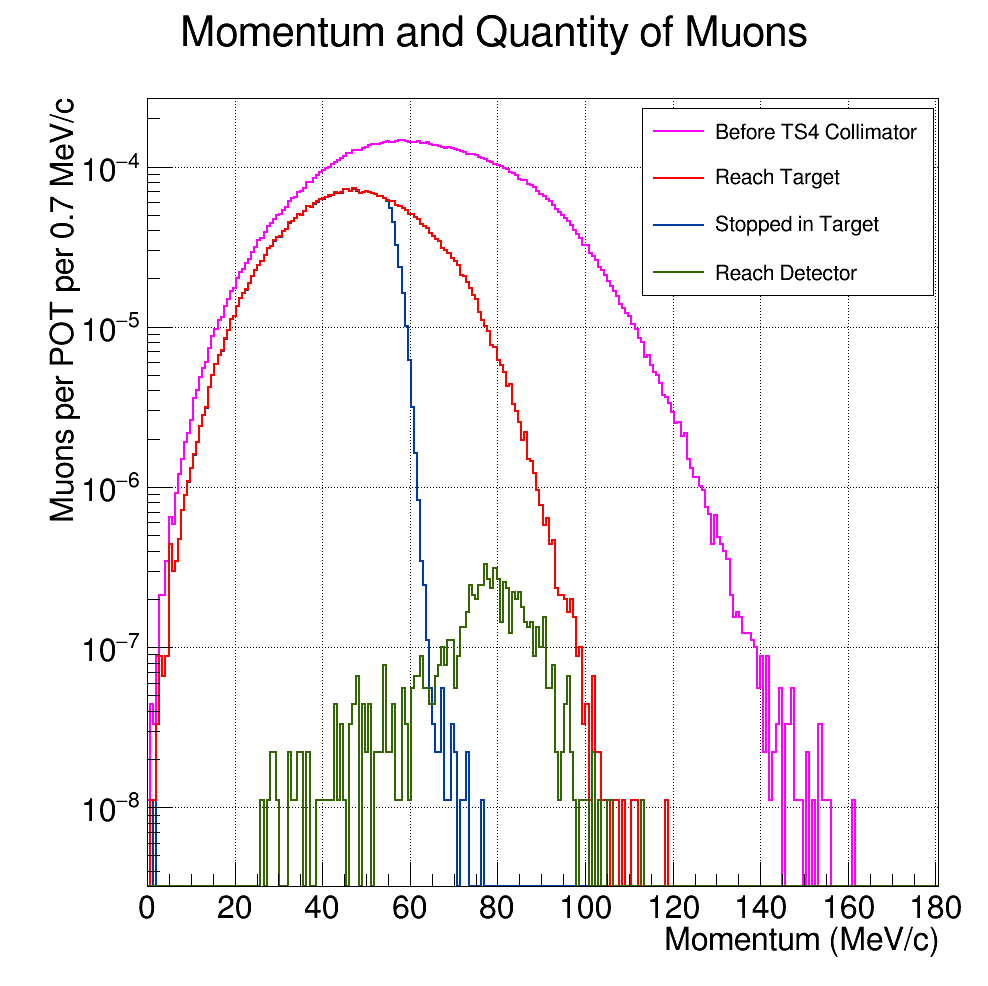
\includegraphics[width=0.49\textwidth,trim=0 0 0 0,clip]{figs/appendixStopTgtImprov/Tidied_muon_momentum_withDetectedMuons_log.png}}
\caption
[The momentum of muons that reach the stopping target and eventually stop.]{
The momentum of muons that reach the stopping target and eventually stop.
By comparison with \fig{sense:muMomenta}, the new target design is clearly able to stop much higher momentum muons, although without the beam blocker
it is also clear that high energy muons reach the detector.
\figlabel{app:tgtImprov:muMomentum}}
\end{figure}
}

\newcommand{\FigTgtImprovSignalDistribution}{
\begin{figure}[tb]
\subfloat[][\figlabel{app:tgtImprov:signalMom:lin}Linear Scale]{%
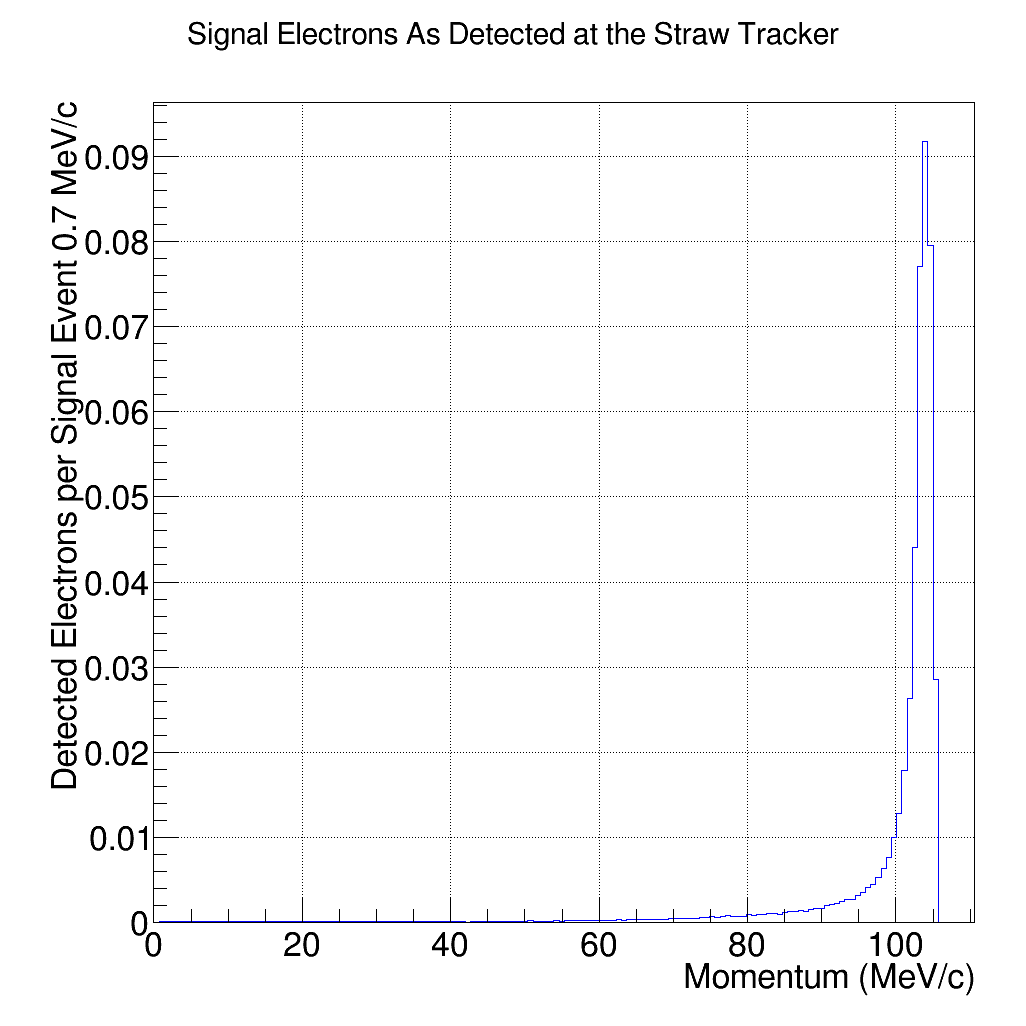
\includegraphics[width=0.49\textwidth,trim=0 0 0 0,clip]{figs/appendixStopTgtImprov/Tidied_StrawTrk_DetectedSignal.png}}
\subfloat[][\figlabel{app:tgtImprov:signalMom:log}Logarithmic Scale]{%
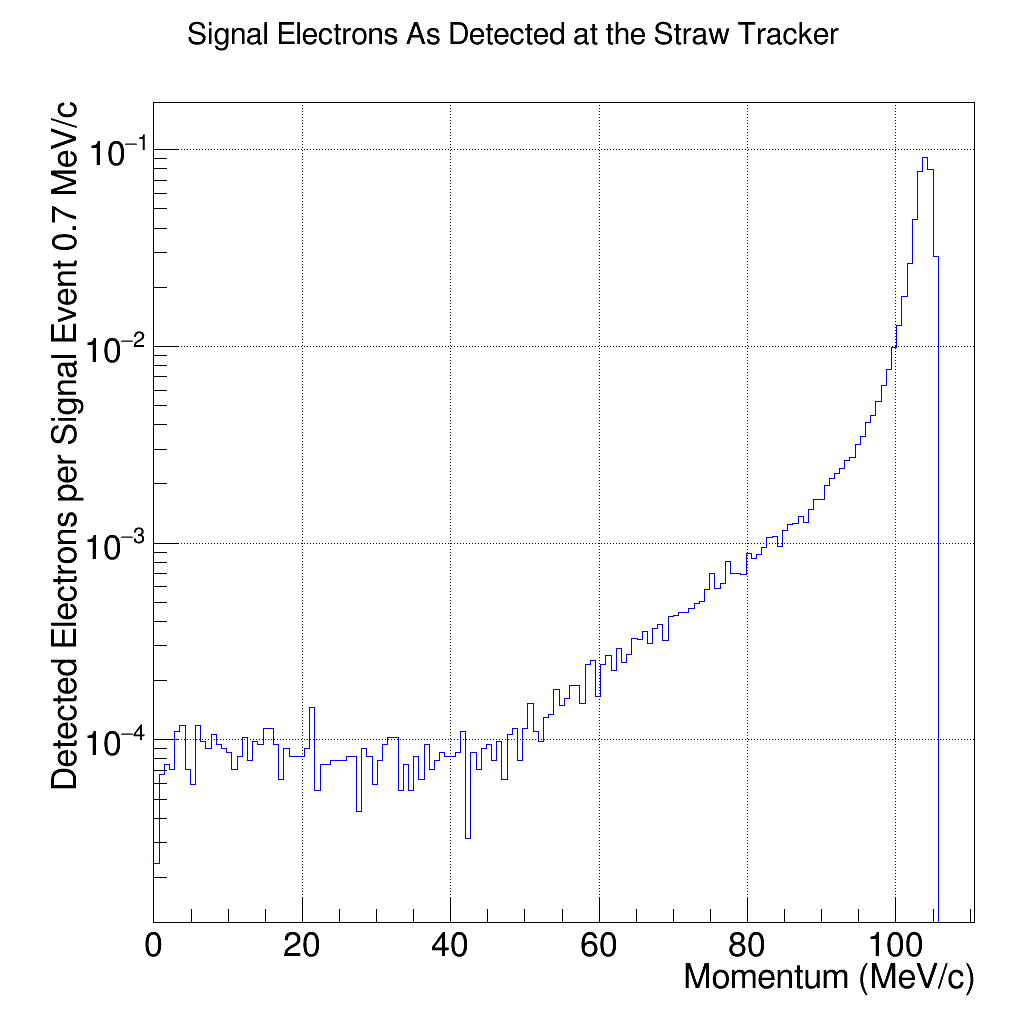
\includegraphics[width=0.49\textwidth,trim=0 0 0 0,clip]{figs/appendixStopTgtImprov/Tidied_StrawTrk_DetectedSignal_log.png}}
\caption
[The observed  momentum distribution and acceptance for signal electrons.]{
The observed  momentum distribution and acceptance for signal electrons.
Given the extra material, the energy losses in the target are larger than the previous design, although the overall geometric acceptance is significantly increased.
\figlabel{app:tgtImprov:signalMom}}
\end{figure}
}

\chapter{Revisiting the Phase-II Stopping Target Region}
\sectlabel{appendix:stopTgtImprove}
Of the various optimisations presented in chapter~\sect{phaseII-optimisation}, the stopping target was only optimised for its position, keeping the shape, thickness and size as in the CDR.
It was also observed in that chapter that the beam blocker had a large impact on the signal acceptance.
To investigate ways in which the sensitivity of \phaseII can be further improved we develop here the idea of a beam blocker-free stopping target design, as well as investigate the impact of changing the target shape.

The overall result of this study suggests an improvement in the signal sensitivity of \phaseII of a factor of 2.5 should be achievable.

\section{Understanding the Stopping Target Region}
\FigTgtImprovFieldVsBeamline
\FigTgtImprovMirrorVsBeamline
\FigTgtImprovGyroradiusVsBeamline
\FigTgtImprovSenseVsBeamline
One of the challenges when optimising the stopping target is the complexity of the region, and correlations between the various parameters.

The magnetic field around the stopping target, for example, is not a simple solenoidal field.
\Fig{app:tgtImprov:field} shows the magnitude of the field along the beamline axis in the stopping target region.
At the exit of the bent solenoids and for the first straight section immediately downstream, the field is kept close to 3~T.
By the entrance of the electron spectrometer, the field on axis is closer to 1~T, although a transverse gradient is introduced from the bent solenoids.
The transition from 3 to 1~T happens over 1.5~m across three solenoid sections.

The stated purpose of the reduction in field strength is to mirror those signal electrons that are produced in the target heading upstream.
This, then, is expected to increase the geometric acceptance of the detector.
Magnetic mirroring can be understood in various ways, such as via the adiabatic constants.
However, qualitatively and intuitively, since magnetic field lines never end (`there are no magnetic monopoles'), when the field strength is reduced, the field lines spread out.
This can be seen as a normal solenoidal field, with a radial component superimposed.
  Normal gyration around the solenoidal field, therefore, generates a Lorentz force that points back along the direction of the solenoidal field, and reduces the longitudinal velocity of the particle.
Thus a particle initially with only transverse momentum in the region of tapering field strength will acquire momentum in the longitudinal direction towards the lower field strength.
Similarly a particle initially heading from a low-magnetic field to a high-magnetic field can be mirrored back if the difference in the field is sufficient.
The limit for this to occur is given by the condition~\cite{Jackson}:
\begin{equation}
\tan^{-1}(\theta)=\left|\frac{v_\mathrm{L}}{v_\mathrm{T}}\right|<\left(\frac{B_\textrm{max}}{B}-1\right)^{1/2},
\end{equation}
where $B_\textrm{max}$ and $B$ are the maximum field strength and current field strength.
$v_\textrm{L}$ and $v_\textrm{T}$ are the longitudinal and transverse velocity of the particle at this point, the ratio of which is the arctangent of the pitch angle, $\theta$, between the particle's velocity and the solenoidal axis.

Given that the maximum field strength occurs at the exit of the Torus2, with a magnitude of $B_\textrm{max}=2.88$~T, one can calculate the minimum pitch angle an upstream-heading particle must have in order for it to be mirrored back downstream.
This is shown in \fig{app:tgtImprov:mirror:thetaMin} where the minimum pitch angle varies from around 85\degree to about 43\degree at the end of Stopping Target Section.
Since signal electrons are produced isotropically, this limit can be turned into the fraction of phase space for signal electrons produced at a point along the beamline that will be mirrored back, and this is shown in \fig{app:tgtImprov:mirror:phaseSpace}.
This clearly motivates putting the stopping target further downstream in order to maximize the mirroring effect.

On the other hand, if the target is located downstream, the muon beam is required to traverse the tapered field.
In that case there is another effect, namely the adiabatic growth of the beam envelope, which must be considered.
Since particles in the beam follow the field lines, as the field is reduced, the beam profile must grow.
This growth is governed by the expression:
\begin{equation}
Ba^2=\textrm{const}
\end{equation}
where $B$ is the field strength at a given point, and $a$ the radius of gyration.
Thus if the field strength reduced by a factor of 4, for example, the beam envelope can be expected to grow by a factor of 2.
The radius of gyration is shown in \fig{app:tgtImprov:gyroradius}, relative to the radius at the exit of the Torus2, as a function of the distance along the beamline.

The position optimisation of the stopping target shown in chapter~\sect{phaseII-optimisation} kept the target disks at a fixed radius and moved the whole set of target disks (and beam blocker) upstream and downstream.
With a fixed radius set of disks, as the target was moved downstream, the fraction of the muon beam expected to hit the target was reduced.
This favoured putting the stopping target more upstream in order to increase muon stopping rate.
%In addition, although it would seem that increasing the target disk radius will mean introducing more material to interfere with signal electrons, the electrons will also experience the same growth in beam size,

Thus there were two competing effects: move the target downstream and the mirroring of signal events increases, but move the target upstream and the muon stopping rate is increased.
These factors can be combined to give a proxy for the expected signal sensitivity for a target disk of fixed radius placed at one point along the beamline.
The muon stopping rate will be proportional to the fraction of the beam profile that overlaps with the target.
Meanwhile, the fraction of upstream-pointing phase space that would be mirrored downstream, plus the fraction of phase space pointing downstream in the first place (half of it), should be proportional to the signal acceptance.
This combination is shown in \fig{app:tgtImprov:senseVsBeamline}.

Indeed, the maxima of this function, at 19700 mm in beamline coordinates, is very close to the optimal location found during the position scan.
This neglects many factors, such as the fact that disks upstream will remove muons from the disks downstream, and that not all electrons that head downstream will be accepted into the detector.
Nevertheless, it seems to capture the underlying phenomena that determine the optimal target location.

\section{Improving the Target Design}
In order to improve the signal acceptance, and taking into account the previous discussion, we make three key changes to the target design.
Firstly we allow the target radius to vary as a function of the beamline distance, thus keeping a constant overlap with the muon beam profile.
Secondly we remove the beam blocker, which will hugely increase the acceptance of signal events.
Finally, to compensate for the missing beam blocker, and to increase the number of stopped muons, we add more target disks into the target.
From \fig{sense:stops} in section~\sect{sense:stops} it can be seen that the muon stopping rate per disk has not reached zero by the last disk, which implies more muons could be stopped.
In addition, the increasing target radius can be used to remove the line of sight between the Torus2 exit and the electron spectrometer that the beam blocker previously provided to remove beam particles.

\FigTgtImprovNewGeom
\TabTgtImprovDiskParams
Although each of these changes should each be studied carefully, as a proof of principle the design shown in the event display in \fig{app:tgtImprov:newGeom} was tested in a simulation.
The disk radii and positions are given in \tab{app:tgtImprov:diskParams}.

To check the sensitivity and stopping rates with this configuration, 75~million POT events were fed in to a simulation that had muon \acf{DIO} and nuclear capture disabled, to be able to study the sensitivity in a single simulation.

\subsection{Muon Stopping Rate}
\FigTgtImprovMuStops
\FigTgtImprovMuMomentum
\FigTgtImprovSignalDistribution
From this simulation, the muon stopping rate was found to be \num{2.8e-3}~per POT, and increase of 1.75 times compared to the stopping rate described in chapter~\sect{sense}.
The stopping distributions in the target are shown in \fig{app:tgtImprov:muStops}.
It can be seen from the projection to the Z-axis that we catch much more of the tail of the distribution.
It can also be seen from the YZ projection how there are very few muons stopping in the upper half of the target. 
This suggests one would really be able to remove this material which would give an additional increase to the signal acceptance.

The extra disks and the enlarged radius also mean that the higher energy muons sitting lower down in the beam are more effectively stopped.
Being at the bottom of the beam these muons were more likely to miss the old target design, but also penetrated further, requiring more target material to be stopped.
This can be seen by comparison of the muon momentum distribution shown in \fig{app:tgtImprov:muMomentum} and comparing this with the momenta shown in \fig{sense:muMomenta}.
Whereas before we only stopped muons up to around 50~MeV/c, now muons up to 60~MeV/c are consistently stopped.
As a result of all of these changes, the stopping efficiency for muons that reach the target has increased from 43\% to about 77\%.

Unfortunately, it can also be seen from \fig{app:tgtImprov:muMomentum} that some of the high-momentum muons that do not stop in the target reach through to the detector.
This means the background rate with the design shown here from beam backgrounds would be significantly larger.
However, further optimisations of the target based on this concept might be able to remove these high-momentum muons using additional disks or adjusting the upstream collimators.

\subsection{Signal Acceptance}
\Fig{app:tgtImprov:signalMom} shows the detected momentum distribution of electrons.
Of the signal events that occur, 48\% are detected at the detector, which is the geometric acceptance with this design, and a factor of 2.2 times better than the result in chapter~\sect{sense}.
The momentum cut however is less efficient now, accepting only 50\% of events, compared to the previous 70\%.  
Overall though, the signal acceptance with this target design is a factor 1.55 times better than the old design.

\subsection{Summary and Future Improvements}
By removing the beam blocker, adding more disks and increasing the disk radius along the beam axis, the muon stopping rate and geometric acceptance increase, although the momentum cut efficiency is decreased.
The overall sensitivity can be expected to increase by a factor of 2.5.

Backgrounds from such a design need to be studied, in particular, high-energy electrons and muons in the beam which are no longer removed by the beam blocker, but should be lost in the target.
In addition the \ac{DIO} background, which given the poorer momentum resolution and greater signal acceptance, might produced more background events with this design, and create a significantly higher hit rate.
Other backgrounds like those from antiprotons in the beam, cosmic rays and neutrons will not be changed by the different stopping target.
Radiative pion capture will be increased slightly since the pion stopping rate will also likely increase.

In addition to background studies with this design there is further optimisation that can be performed.
The most obvious area for improvement is to remove the material at the top part of the target disks, since in this region no muons stop here.
In addition one can add more target disks to the lower part to try and catch even more of the high-momentum tail.

The target disk thickness is another parameter that could be studied.
In fact, somewhere between these two options is the possibility to use wedge-shaped target disks, that put less material higher up in the beam.
If one can control this so that the low-momentum muons stop as far downstream as possible, rather than in the first target disk, as currently occurs, then one can improve both the signal acceptance \emph{and} the momentum resolution.
